
% this file is called up by thesis.tex
% content in this file will be fed into the main document

%: ----------------------- introduction file header -----------------------
\chapter{Introducció}\label{cap:int}

% the code below specifies where the figures are stored
\ifpdf
    \graphicspath{{1_introduction/figures/PNG/}{1_introduction/figures/PDF/}{1_introduction/figures/}}
\else
    \graphicspath{{1_introduction/figures/EPS/}{1_introduction/figures/}}
\fi

% ----------------------------------------------------------------------
%: ----------------------- introduction content ----------------------- 
% ----------------------------------------------------------------------



%: ----------------------- HELP: latex document organisation
% the commands below help you to subdivide and organise your thesis
%    \chapter{}       = level 1, top level
%    \section{}       = level 2
%    \subsection{}    = level 3
%    \subsubsection{} = level 4
% note that everything after the percentage sign is hidden from output

Aquesta memòria pretén reflectir de manera clara i entenedora el procés que s'ha seguit per dur a terme un laboratori de "Sistemes Distribuïts de Control" (a partir d'ara SDC), així com els problemes que hagin pogut sorgir en el transcurs del projecte.

La realització d'aquest laboratori ha comportat l'adquisició d'una visió profunda del que es pretén ensenyar des del departament de ESAII \index{ESAII} de la UPC en el tema dels SDC \index{SDC}.

Per tant en el transcurs d'aquesta memòria s'anirà endinsant en aquest tipus de sistemes, es coneixeran quines són algunes de les tecnologies base que els conformen, els problemes que en elles esdevenen, i solucions a algunes d'aquestes qüestions.

Amb tot això es podrà tenir una idea més clara del motiu de la realització d'aquest projecte i les portes que a partir d'aquest projecte queden obertes.

A més es poden veure com a apèndix les dues guies realitzades en aquest projecte, una per la preparació de l'entorn de desenvolupament i posterior utilització del laboratori. I una altre per l'ús del LiveCD \index{LiveCD} pel desenvolupament pràctic del laboratori.

%====================================================================================%
% Estructuració de la memòria
%====================================================================================%
\section{Estructuració de la memòria}\label{cap:int:estruct}

En aquesta secció mirarem de donar una visió global de la memòria, perquè sigui fàcil de ser consultada, i d'aquesta manera tenir en tot moment una idea de on es pot trobar qualsevol qüestió. Per tant començar indicant que aquesta memòria ha estat escrita seguint l'ordre cronològic que esdevé al desenvolupar i portar a terme un projecte.

D'aquesta manera primerament ens trobem  amb el capítol de Introducció (capítol \ref{cap:int}), en el qual podem veure resumidament de que tracta el projecte, quines són les raons de la seva elecció i perquè aquest projecte és important (secció Motivació \ref{cap:int}), quin era l'objectiu d'aquest projecte amb les limitacions del temps que tenia (secció Abast \ref{cap:int:ab}), i de quina manera es va organitzar el temps per realitzar-lo, i reorganitzar-lo en el moment que això va caldre (secció Planificació \ref{cap:int:plan}).

Un cop es té una idea global ben clara dels objectius d'aquest projecte, és el moment d'aprofundir una mica en les tecnologies que en aquest es toquen, per tant tot seguit veurem el capítol Tecnologia (capítol \ref{cap:tec}). Aquest capítol l'hem dividit en tres parts per tipus de tecnología. 

En la primera part parlarem sobre els dispositius físics (secció Hardware \ref{cap:tec:hard}) en la que explicarem quines plaques s'utilitzen al laboratori per fer els controls (secció FLEX \ref{cap:tec:hard:flex}), tot seguit explicarem quin es el nucli d'aquestes plaques (secció dsPIC33FJ256MC710 \ref{cap:tec:hard:dspic}), quin integrat ens permet fer d'intermediari per les comunicacions CAN (secció MCP2551 \ref{cap:tec:hard:mcp2551}), i amb quin dispositiu podem programar qualsevol microcontrolador de la casa Microchip (secció ICD2/3 \ref{cap:tec:hard:icd}).

En la segona part parlarem del software que s'ha usat per elaborar el projecte i el laboratori (secció Software \ref{cap:tec:soft}), en ella parlarem del IDE que hem utilitzat per programar tant el codi en python del programa \DCSMonitor com el codi del Sistema Operatiu en Temps Real Erika (secció \Eclipse \ref{cap:tec:soft:eclipse}), el programa que hem utilitzat per programar els dispositius (secció \MplabX \ref{cap:tec:soft:mplab}), del IDE que hem usat per crear les interficies del programa \DCSMonitor (secció QtCreator \ref{cap:tec:soft:qtcreator}), de la eina que ens facilita crear els fitxers de traducció del programa \DCSMonitor (secció QtLingüist \ref{cap:tec:soft:qtlinguist}), i per ultim el Sistema Operatiu en Temps Real que formen el cervell dels dispositius del bus CAN (secció ERIKA Enterprise \ref{cap:tec:soft:erika}).

Per ultim farem una pinzellada a alguns protocols que hem d'entendre per poder ser conscients dels problemes i solucions que atorga cadascun (secció Protocols de comunicació \ref{cap:tec:prot}), així que comencem per el més important en els Sistemes Distribuits de Control amb el qual tots els dispositius es troben ben comunicats (secció CAN ref{cap:tec:prot:can}), tot seguit el que ens permet rebre a l'ordinador tot el que está succein al bus CAN (secció Serie via RS232 \ref{cap:tec:prot:rs232}), i per finalitzar el tipus de topologia en el que es troben tots els dispositius del laboratori (secció Topologia en bus \ref{cap:tec:prot:bus})

A partir d'aquest punt comença a aparèixer les noves idees que aporta el projecte, en el capítol Disseny del laboratori (capítol \ref{cap:dis}) primerament s'explicarà que s'ensenya actualment en el laboratori, i quines són les eines que s'utilitzen (secció Resum del laboratori actual ,\ref{cap:dis:resum}). Tot seguit amb la secció Disseny del Nou laboratori ,\ref{diss:nou}, es plantegen quins són els problemes que es volen resoldre, i com s'aconsegueix en alguns temes del laboratori com són la creació de la interfície (secció \ref{cap:dis:visual}), els problemes amb els identificadors que s'han d'assignar als diferents dispositius del bus CAN (secció \ref{cap:dis:idCAN}), la comunicació entre el programa \DCSMonitor (programa que corre a l'ordinador) i els diferents dispositius mitjançant comunicació serie per RS232 (secció \ref{cap:dis:comSer}), el disseny que es va pensar pel mostreig de les gràfiques en temps real (secció \ref{cap:dis:graph}) i el mètode escollit per poder fer el programa multilingüe i fàcilment ampliable (secció \ref{cap:dis:idi}).

Per altre banda tenim el \emph{com} es va portar a terme el sistema dissenyat anteriorment, d'aquesta manera en el capítol Implementació del laboratori (capítol \ref{cap:imp}) toca el torn d'explicar la metodología per fer realitat el laboratori plantejat. 
Primerament ens centrarem en el programa d'ordinador \DCSMonitor (secció \ref{cap:imp:dcs}) començant per la part visual del programa (la interfície en la secció \ref{cap:imp:visual}), seguint amb la implementació de la comunicació sèrie (secció \ref{cap:imp:com:serie}). Després una de les parts més importants que és la generació de les gràfiques en temps real (secció \ref{cap:imp:gen:graph}); gracies a les quals podem avaluar la bondat dels controls que hi ha al bus CAN, l'exportació d'aquestes gráfiques en diferents formats (secció \ref{cap:imp:exp:graph}) i finalment la integració de la multiculturalitat, o creació de la interficie multilingüe (secció \ref{cap:imp:idi}).
La part dels dispositius no és menys important, i per tant té també la seva secció d'implementació (\ref{lab:imp:dspic:monitor}), en ella s'expliquen els mètodes que s'han usat per portar a terme les comunicacions series per RS232 (secció \ref{lab:imp:dspic:monitor:serie}), i tot el relacionat amb les comunicacions CAN (secció \ref{lab:imp:dspic:can}).


Al acabar el projecte, ha estat possible comprovar les hores reals que si han dedicat, i per tant fer càlculs dels preus del material i de la ma d'obra. Per tant tot seguit ve el capítol Anàlisi econòmic \ref{cap:eco}, on es poden veure un desglos del preu del projecte.

Després venen les conclusions ,\ref{cap:conc}, on es deixa constància de quins han estat els objectius aconseguits, possibles ampliacions que pot tindre aquest projecte, i una visió general després d'haver realitzat el projecte.


Com apèndix tenim les dues guies que s'han elavorat per l'execució del laboratori en un sistema Linux (\Ubuntu) \ref{cap:lab_gui}, i una guia d'us del \LiveCD creat en aquest projecte, per tenir en marxa tot aquest sistema en 6 minuts (més larrancada de l'ordinador) \ref{cap:cd_gui}.


%====================================================================================%
% Motivació
%====================================================================================%
\section{Motivació}\label{cap:int:mot}

Moltes són les raons per les quals aquest projecte va ser començat i posteriorment tirat endavant. Primerament perquè els sistemes electrònics empotrats són a tot arreu; caixers automàtics, impressores, calculadores, rellotges, equips mèdics, telèfons mòbils... Però què és un sistema si no pot ser consultat en temps real? De que serveix un sistema electrònic aïllat del que no es pot treure cap tipus d'informació a l'instant? Actualment quasi tots els sistemes procuren d'una o altre manera estar en constant comunicació, volem saber en cada moment quin és l'estat d'alguna lectura, si hi ha algun problema en algun aparell que hagi de ser revisat, si el ABS del cotxe funcionarà en el moment que toqui, si el cafè de després de les postres ja és ben calent... 
 
Per tant l'aparició dels sistemes distribuïts es veu forçada a sorgir de les mancances que tenien els sistemes totalment autònoms, i així esdevenir poc a poc una realitat actual. Peró aquesta aparició no sorgeix i esdevé una realitat idíl·lica en el moment de néixer, sinó que junt amb ella apareixen nous problemes e inconvenients; la concurrència de tots els sistemes comunicats és un problema greu, i no tots els sistemes són igual de crítics; n'hi ha que només donen lectures periòdiques sense massa importància, però també n'hi ha que salven vides.

Un clar exemple de tot això és el protocol de comunicació CAN, desenvolupat fa només 3 dècades; aquest va començar a l'any 1983 per \emph{Robert Bosch GmbH} i va ser oficialment alliberat al 1986 per la Societat d'Enginyers Automotrius (SAE, Society of Automotive Engineers). Va ser principalment creat per la industria automòbil, gracies a la qual es van poder posar molts dels sistemes de seguretat que hi ha actualment als cotxes; gracies als quals es salven moltes vides; però que actualment és usat en molts altres sectors, com poden ser equips mèdics, controls industrials, entorns aeroespacials, marítims, etc.

Aquesta és una de les raons per les quals s'ha escollit la realització d'aquest projecte. Perquè són sistemes reals, i que encara no estan perfeccionats; i això és així no perquè no siguin importants, sinó perquè pertanyen a una branca de la tecnologia que encara està en constant evolució.

Per tant, espero que es vegi la importància que aquest projecte porta darrera, i que la realització d'aquest no tanca cap porta, sinó que deixa obert un camí molt llarg per explorar.


%====================================================================================%
% Abast
%====================================================================================%
\section{Abast}\label{cap:int:ab}

Aquest projecte pot ser continuat, per tant cal indicar que amb la limitació de temps amb la que conta el projecte (relativa al nombre de crèdits), en algun moment s'ha hagut de posar una fita. Per tant s'exposa en aquest apartat els objectius que s'han proposat aconseguir.


%====================================================================================%
% Objectius
%====================================================================================%
\subsection{Objectius}% subsection headings are again smaller than section names
% lead
Abans  d'escollir aquest projecte es van plantejar alguns dels objectius que aquest hauria de complir, però un cop començat es van anar refinant i ampliant fins arribar a generar una idea més específica d'aquests. Per tant tot seguit es mostren els objectius que finalment es van decidir:
\begin{enumerate}
	\item Adaptar codi existent en el “Laboratori de Sistemes Distribuïts de Control” del màster en “Automàtica i Robòtica” del departament del ESAII per poder-lo realitzar completament amb Software Lliure.
	\item Dissenyar un laboratori de Sistemes Distribuïts de Control executable amb Software Lliure. Aquest laboratori ha de poder comprovar el bon funcionament del treball dels diferents alumnes, i per fer aquesta tasca s'han de crear varis programes:
		\begin{enumerate}
			\item Programa per ordinador amb dos modes d'execució (\DCSMonitor).
				\begin{enumerate}
					\item Mode Monitor.
						\begin{itemize}
							\item S'ha de poder connectar amb una placa Flex monitora via RS232.
							\item Ha de poder llistar els diferents llaços de control que hi hagi al bus CAN al que estigui connectat la placa Flex monitora.
							\item Ha de ser capaç de rebre tota la informació necessària per avaluar la qualitat dels diferents algoritmes de control que estiguin executant els alumnes.
							\item Capaç de dibuixar les gràfiques en temps real del control que estiguin executant els diferents llaços.
							\item Ha de poder generar càrrega al bus CAN per observar els problemes que apareixen quan un bus amb aquest protocol es satura.
						\end{itemize}
					\item Mode Sensor/Actuador.
						\begin{itemize}
							\item Ha de ser capaç de rebre la informació del \SensorActuador que envia l'estat de les seves senyals.
							\item Ha de poder generar la gràfica en temps real del control que s'està efectuant.
						\end{itemize}
					\item Opcions compartides.
						\begin{itemize}
							\item Multilingüe.
							\item Poder afegir o eliminar de la gràfica alguna de les línies (referencia, valor d'entrada, primera i/o segona integral) en temps real, o un cop la imatge fos aturada.
							\item Poder generar una imatge amb varies opcions:
								\begin{itemize}
									\item En varis formats.
									\item Autocontinguda amb tota la informació necessària (títol del laboratori, subtítol, llegenda).
									\item Amb els plots que es desitgin (referencia, valor d'entrada, primera i/o segona integral).
									\item Amb tots els textos de la gràfica multilingüe.
								\end{itemize}
						\end{itemize}
				\end{enumerate}
			\item Programa monitor per un microcontrolador.
				\begin{itemize}
					\item Ha de poder guardar quins dispositius hi ha al bus CAN.
					\item Ha de ser capaç d'interferir en les comunicacions del bus CAN.
					\item Ha de poder capturar l'estat d'un llaç de control.
					\item Ha de poder enviar tota aquesta informació al programa d'ordinador mitjançant comunicació sèrie per RS232.
					\item Ha de poder rebre ordres del programa d'ordinador mitjançant la comunicació sèrie per RS232.'
				\end{itemize}
			\item Programa Controlador per un microcontrolador.
				\begin{itemize}
					\item Ha de ser capaç de rebre l'estat del Sensor.
					\item Ha de calcular el senyal a aplicar al doble integrador tenint en compte la discretització dels temps.
					\item Ha d'enviar el senyal d'entrada del doble integrador l'\Actuador.
				\end{itemize}
			\item Programa \SensorActuador per un microcontrolador.
				\begin{itemize}
					\item Ha de ser capaç de llegir l'estat de la primera i segona integral.
					\item Ha d'enviar els valors de la primera i segona integral al Controlador.
					\item Ha de rebre el senyal a aplicar del controlador.
					\item Ha de poder enviar tota aquesta informació al programa d'ordinador mitjançant comunicació sèrie per RS232.
				\end{itemize}
		\end{enumerate}
	\item Implementar el laboratori mencionat al punt anterior.
	\item Realitzar la documentació necessària per tenir l'entorn de desenvolupament i posta en marxa de tot el sistema multilingüe.
	\item Preparar l'entorn Live CD amb tot el material necessari per realitzar l'execució del laboratori.
	\item Preparar una guia d'ús multilingüe del Live CD.
\end{enumerate}



%====================================================================================%
% Planificació
%====================================================================================%
\section{Planificació}\label{cap:int:plan}

La planificació del projecte va ser en un principi una aproximació de la feina que s'havia de realitzar, ajustada al temps que oferien el nombre de crèdits a realitzar, però en aquesta estimació no hi havia inconvenients temporals i per tant era un esquema totalment idíl·lic.

\begin{center}
	\begin{tabular}{ c | c | c | c | c | c }
		\textbf{crèdits} & \textbf{crèdit/hora} & \textbf{hores} & \textbf{hores/dia} & \textbf{dies} & \textbf{mesos}\\
		\hline
		22,5 & 20 & 450 & 5 & 90 & ~4.5\\
		\hline
	\end{tabular}
	\captionof{table}{Estimació de la duració del projecte}
	\label{tab:int:plan:est:temps}
\end{center}

D'aquesta manera, al iniciar el projecte el 20 de Juny i havent realitzat els càlculs del temps a dedicar (taula \ref{tab:int:plan:est:temps}) es preveia que al voltant de Novembre el projecte ja estaria finalitzat, i es podria procedir a fer la lectura d'aquest. 
Un cop posada la fita i les hores a dedicar, es va assignar les hores a les diferents tasques que s'esperava realitzar, per d'aquesta manera veure si el projecte s'ajustava correctament a aquestes hores (taula \ref{tab:int:plan:hores}). I tenint en compte la taula de hores diàries vista anteriorment, ens surten els dies i hores que aquí apareixen.
Així doncs es va ajustar la feina al calendari i efectivament tot encaixava, però a finals d'Agost per problemes personals el projecte es va haver d'aturar completament, i això es va allargar un mes i mig. Això va causar una replanificació del diagrama de gantt i l'entrega del projecte es va veure afectada en una demora equivalent a aquest temps (es pot observar en el diagrama de gantt (Principi del gantt \ref{gantt_nuevo_v_pag1} i \ref{gantt_nuevo_v_pag2}) el període de demora esmentat).


% per preparar bé les seccions de la planificacio s'ha d'executar el canvi per
% expresio regular :^([0-9]+) &([^\n]+)&([^\n]+)\\\\
% per el següent   :\\textbf{\1} & \\textbf{\2} & \\textbf{\3}\\\\
\begin{center}
	\begin{longtable}{ l | p{10cm} | r }
		%%%%%%%%%%%%%%%%%%%%%%%%%%%%%%%%%%%%%%%%%%%%%%%%%%%%%%%%%%%%%%%%%%%%%%%
%%                                                                  %%
%%  This is a LaTeX2e table fragment exported from Gnumeric.        %%
%%                                                                  %%
%%%%%%%%%%%%%%%%%%%%%%%%%%%%%%%%%%%%%%%%%%%%%%%%%%%%%%%%%%%%%%%%%%%%%%
WBS	&Nombre	&Trabajo\\
\hline
1	&Estudi General	&3d 4h\\
\hline
1.1	&Buscar informaci� ROTS	&1d 4h\\
\hline
1.2	&Mirar Erika ROTS	&1d\\
\hline
1.3	&Mirar Comunicaci� CAN bus	&1d\\
\hline
2	&Planificar Projecte	&4h\\
\hline
2.1	&Planificaci� general del projecte	&4h\\
\hline
3	&Laboratori Actual	&28d 4h\\
\hline
3.1	&Mirar material necessari	&7h\\
\hline
3.2	&Preparar i adaptar entorn de treball	&2d 4h\\
\hline
3.3	&Practica Encendre Led	&1d\\
\hline
3.4	&Practica Doble Integrador	&2d 5h\\
\hline
3.5	&Practica Controlador - Actuador	&2d 2h\\
\hline
3.6	&Recopilar informacio per la FAQ	&9d 4h\\
\hline
3.7	&Recopilar informaci� sobre els passos seguits	&9d 4h\\
\hline
4	&Preparar Codis Lliures	&6d 2h\\
\hline
4.1	&Estudiar la comunicaci� per RS232 amb PIC	&1d\\
\hline
4.2	&Mirar comunicaci� per RS232 amb python	&2d 2h\\
\hline
4.3	&Mirar llibreries per fer gr�fiques amb python	&2d 7h\\
\hline
5	&Realitzar Ampliaci� del Laboratori	&26d 6h\\
\hline
5.1	&Disenyar primera aproximaci� ampliaci�	&1d\\
\hline
5.2	&Implementaci� primera aproximaci�	&4d\\
\hline
5.2.1	&Implementar part Sampling, Actuation	&1d 4h\\
\hline
5.2.2	&Implementar part Control, Monitor	&1d\\
\hline
5.2.3	&Implementar part Receptor (PC)	&1d 4h\\
\hline
5.3	&Replanificar i reorganitzar	&1d 1h\\
\hline
5.4	&Re-disenyar ampliaci�	&5d 6h\\
\hline
5.4.1	&Pensar resultat esperat	&1d 5h\\
\hline
5.4.2	&Dise�ar parts implicades	&2d\\
\hline
5.4.3	&Especificar protocols de comunicaci�	&2d\\
\hline
5.5	&Implementaci�	&12d 5h\\
\hline
5.5.1	&Implementar part Sampling, Actuation	&7h\\
\hline
5.5.2	&Impementar part Control	&1d\\
\hline
5.5.3	&Implementar part Monitor	&3d 6h\\
\hline
5.5.4	&Implementar part Receptor	&3d 5h\\
\hline
5.5.4.1	&Diseny de la part visual	&1d 1h\\
\hline
5.5.4.2	&Integraci� amb comunicaci�	&1d\\
\hline
5.5.4.3	&Mostreig de resultats en temps real	&1d 4h\\
\hline
5.5.5	&Realitzar tests	&2d\\
\hline
5.5.6	&Depuraci� de codi	&1d 2h\\
\hline
5.6	&Documentar nou laboratori	&1d 1h\\
\hline
5.7	&Traduir al Angl�s nou laboratori	&1d\\
\hline
6	&Preparar Live CD	&7d\\
\hline
6.1	&Estudi de la creaci�	&2d\\
\hline
6.2	&Creaci� d'entorn	&1d 4h\\
\hline
6.3	&Implementar Live CD	&7h\\
\hline
6.4	&Revisar bon funcionament	&1d 4h\\
\hline
6.5	&Documentar us del CD	&1d\\
\hline
7	&Realitzar Guia Laboratori	&4d 6h\\
\hline
7.1	&Realitzar guia Catal�	&3d 6h\\
\hline
7.1.1	&Instalaci� entorn	&7h\\
\hline
7.1.1.1	&Linux (ubuntu)	&7h\\
\hline
7.1.2	&Configuraci� entorn	&6h\\
\hline
7.1.2.1	&Linux (ubuntu)	&6h\\
\hline
7.1.3	&Realitzar la guia de seguiment del laboratori	&2d\\
\hline
7.2	&Traduir guia al Angl�s	&1d\\
\hline
8	&Preparar Informe previ del projecte	&3d 4h\\
\hline
9	&Entrega Informe previ del projecte	&\\
\hline
10	&Preparar Mem�ria	&28d\\
\hline
11	&Preparar Defensa	&3d 4h\\
\hline
12	&Reunions peri�diques	&78d 3h\\
\hline
13	&Defensa del projecte	&\\
\hline

		
%%%%%%%%%%%%%%%%%%%%%%%%%%%%%%%%%%%%%%%%%%%%%%%%%%%%%%%%%%%%%%%%%%%%%%
%%                                                                  %%
%%  This is a LaTeX2e table fragment exported from Gnumeric.        %%
%%                                                                  %%
%%%%%%%%%%%%%%%%%%%%%%%%%%%%%%%%%%%%%%%%%%%%%%%%%%%%%%%%%%%%%%%%%%%%%%
\textbf{WBS} & \textbf{Nom} & \textbf{Temps}\\
\hline \hline
	\textbf{1} & 		\textbf{Estudi General } & 	\textbf{3d 4h}\\
\hline
1.1 & Buscar informació RTOS & 1d 4h\\
\hline
1.2 & Mirar Erika RTOS & 1d\\
\hline
1.3 & Mirar Comunicació CAN bus & 1d\\
\hline \hline
	\textbf{2} & 	\textbf{Planificar Projecte } & 	\textbf{4h}\\
\hline
2.1 & Planificació general del projecte & 4h\\
\hline \hline
	\textbf{3} & 	\textbf{Laboratori Actual } & 	\textbf{28d 4h}\\
\hline
3.1 & Mirar material necessari & 7h\\
\hline
3.2 & Preparar i adaptar entorn de treball & 2d 4h\\
\hline
3.3 & Practica Encendre Led & 1d\\
\hline
3.4 & Practica Doble Integrador & 2d 5h\\
\hline
3.5 & Practica Controlador - Actuador & 2d 2h\\
\hline
3.6 & Recopilar informació per la FAQ & 9d 4h\\
\hline
3.7 & Recopilar informació sobre els passos seguits & 9d 4h\\
\hline \hline
	\textbf{4} & 	\textbf{ Preparar Codis Lliures } & 	\textbf{6d 2h}\\
\hline
4.1 &  Estudiar la comunicació per RS232 amb PIC & 1d\\
\hline
4.2 &  Mirar comunicació per RS232 amb python & 2d 2h\\
\hline
4.3 &  Mirar llibreries per fer gràfiques amb python & 2d 7h\\
\hline \hline
	\textbf{5} & 	\textbf{ Realitzar Ampliació del Laboratori } & 	\textbf{26d 6h}\\
\hline
5.1 & Dissenyar primera aproximació ampliació & 1d\\
\hline
5.2 & Implementació primera aproximació & 4d\\
\hline
5.2.1 & Implementar part Sampling, Actuation & 1d 4h\\
\hline
5.2.2 & Implementar part Control, Monitor & 1d\\
\hline
5.2.3 & Implementar part Receptor (PC) & 1d 4h\\
\hline
5.3 & Replanificar i reorganitzar & 1d 1h\\
\hline
5.4 & Redissenyar ampliació & 5d 6h\\
\hline
5.4.1 & Pensar resultat esperat & 1d 5h\\
\hline
5.4.2 & Dissenyar parts implicades & 2d\\
\hline
5.4.3 & Especificar protocols de comunicació & 2d\\
\hline
5.5 & Implementació & 12d 5h\\
\hline
5.5.1 & Implementar part Sampling, Actuation & 7h\\
\hline
5.5.2 & Implementar part Control & 1d\\
\hline
5.5.3 & Implementar part Monitor & 3d 6h\\
\hline
5.5.4 & Implementar part Receptor & 3d 5h\\
\hline
5.5.4.1 & Disseny de la part visual & 1d 1h\\
\hline
5.5.4.2 & Integració amb comunicació & 1d\\
\hline
5.5.4.3 & Mostreig de resultats en temps real & 1d 4h\\
\hline
5.5.5 & Realitzar tests & 2d\\
\hline
5.5.6 & Depuració de codi & 1d 2h\\
\hline
5.6 & Documentar nou laboratori & 1d 1h\\
\hline
5.7 & Traduir al Anglès nou laboratori & 1d\\
\hline \hline
	\textbf{6} & 	\textbf{Preparar Live CD } & 	\textbf{7d}\\
\hline
6.1 & Estudi de la creació & 2d\\
\hline
6.2 & Creació d'entorn & 1d 4h\\
\hline
6.3 & Implementar Live CD & 7h\\
\hline
6.4 & Revisar bon funcionament & 1d 4h\\
\hline
6.5 & Documentar ús del CD & 1d\\
\hline \hline
	\textbf{7} & 	\textbf{Realitzar Guia Laboratori } & 	\textbf{4d 6h}\\
\hline
7.1 & Realitzar guia Català & 3d 6h\\
\hline
7.1.1 & Instal·lació entorn & 7h\\
\hline
7.1.1.1 & Linux (ubuntu) & 7h\\
\hline
7.1.2 & Configuració entorn & 6h\\
\hline
7.1.2.1 & Linux (ubuntu) & 6h\\
\hline
7.1.3 & Realitzar la guia de seguiment del laboratori & 2d\\
\hline
7.2 & Traduir guia al Anglès & 1d\\
\hline \hline
	\textbf{8} & 	\textbf{Preparar Informe previ del projecte } & 	\textbf{3d 4h}\\
\hline \hline
\textbf{9} & \textbf{Entrega Informe previ del projecte} & \\
\hline \hline
	\textbf{10} & 	\textbf{Preparar Memòria } & 	\textbf{28d}\\
\hline \hline
	\textbf{11} & 	\textbf{Preparar Defensa } & 	\textbf{3d 4h}\\
\hline \hline
	\textbf{12} & 	\textbf{Reunions periòdiques } & 	\textbf{78d 3h}\\
\hline \hline
\textbf{13} & \textbf{Defensa del projecte} & \\
\hline
		
	\caption{Hores de dedicació}
	\label{tab:int:plan:hores}
	\end{longtable}

\end{center}

\begin{figure}[p]% will be the left-side figure
	\begin{leftfullpage}
		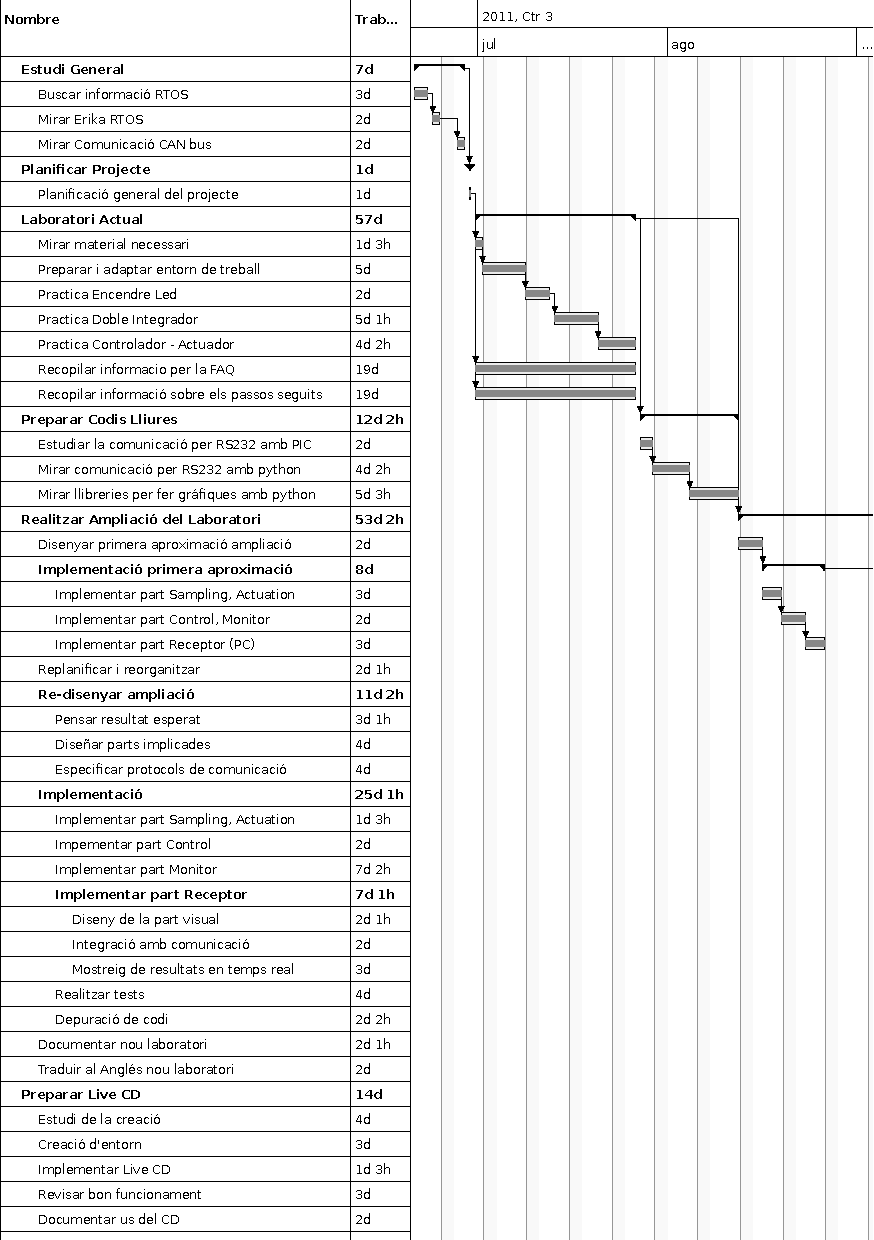
\includegraphics[width=1\textwidth]{gantt_nuevo_v_pag1}
	\end{leftfullpage}
	\caption[Principi del Gantt, esquerre]{\textbf{Principi del Gantt, esquerre} : Juny, Juliol, Agost}
	\label{gantt_nuevo_v_pag1}
\end{figure}
\begin{figure}[p]% will be the right-side figure
	\begin{fullpage}
		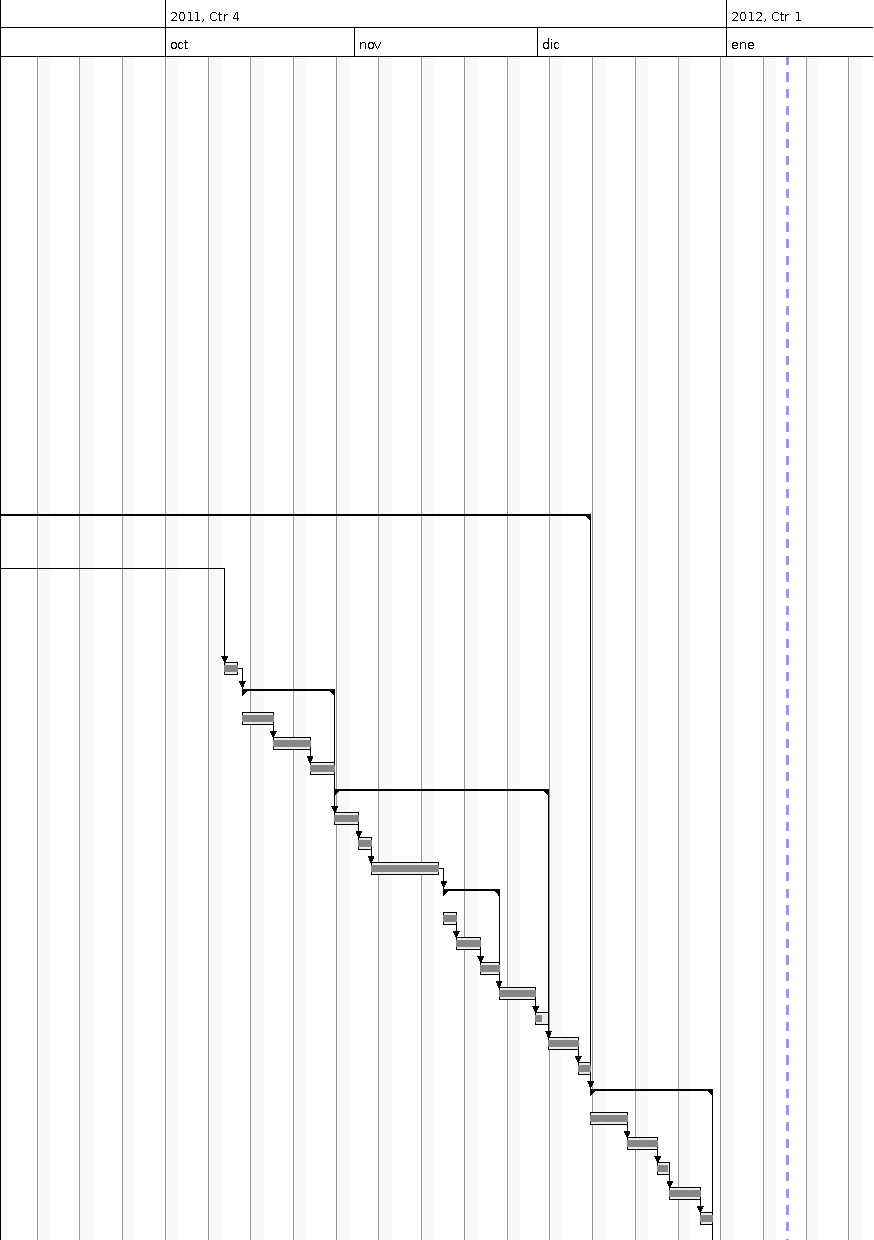
\includegraphics[width=1\textwidth]{gantt_nuevo_v_pag2}
	\end{fullpage}
	\caption[Principi del Gantt, dreta]{\textbf{Principi del Gantt, dreta} : Septembre, Octubre, Novembre, Desembre, Gener}
	\label{gantt_nuevo_v_pag2}
\end{figure}

\begin{figure}[p]% will be the left-side figure
	\begin{leftfullpage}
		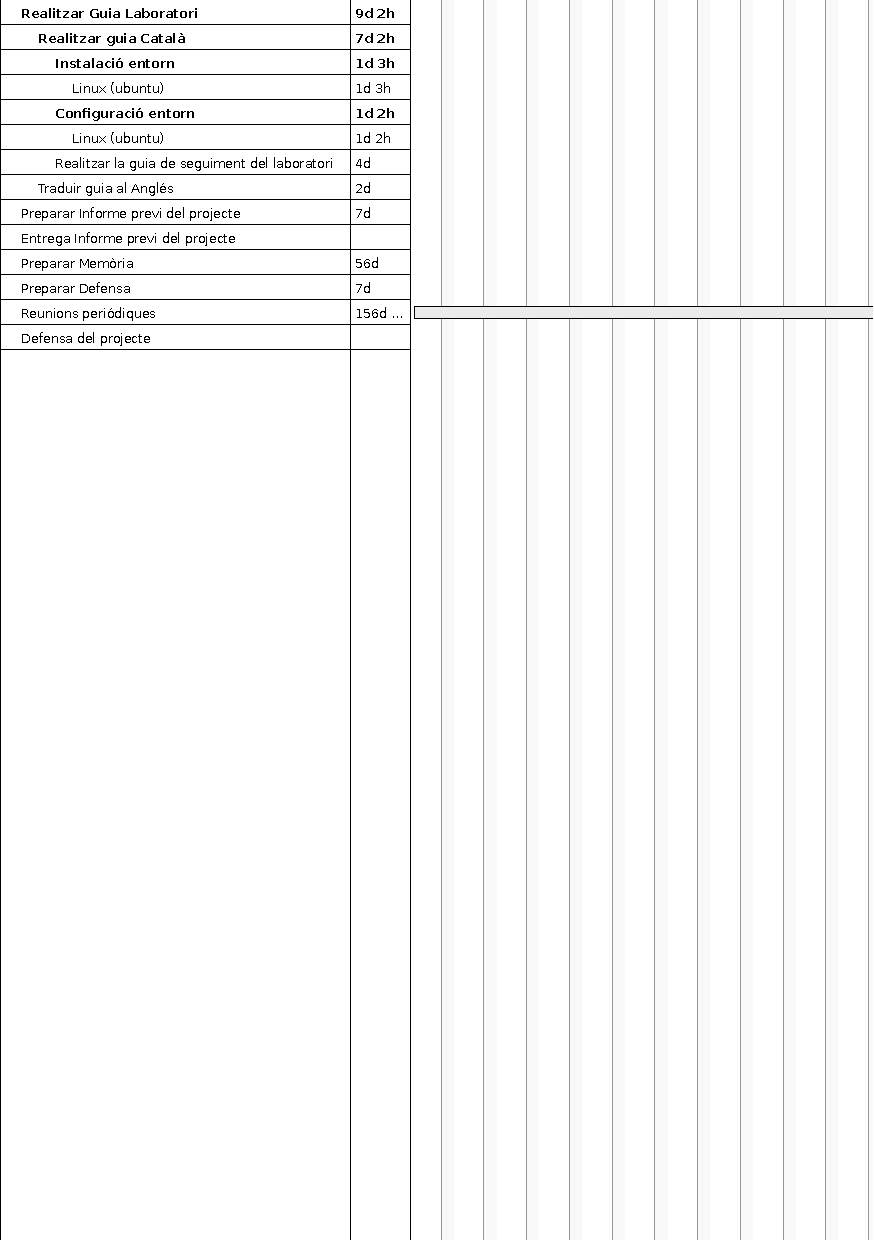
\includegraphics[width=1\textwidth]{gantt_nuevo_v_pag3}
	\end{leftfullpage}
	\caption[Final del Gantt, esquerre]{\textbf{Final del Gantt, esquerre} : Juny, Juliol, Agost}
	\label{gantt_nuevo_v_pag3}
\end{figure}
\begin{figure}[p]% will be the right-side figure
	\begin{fullpage}
		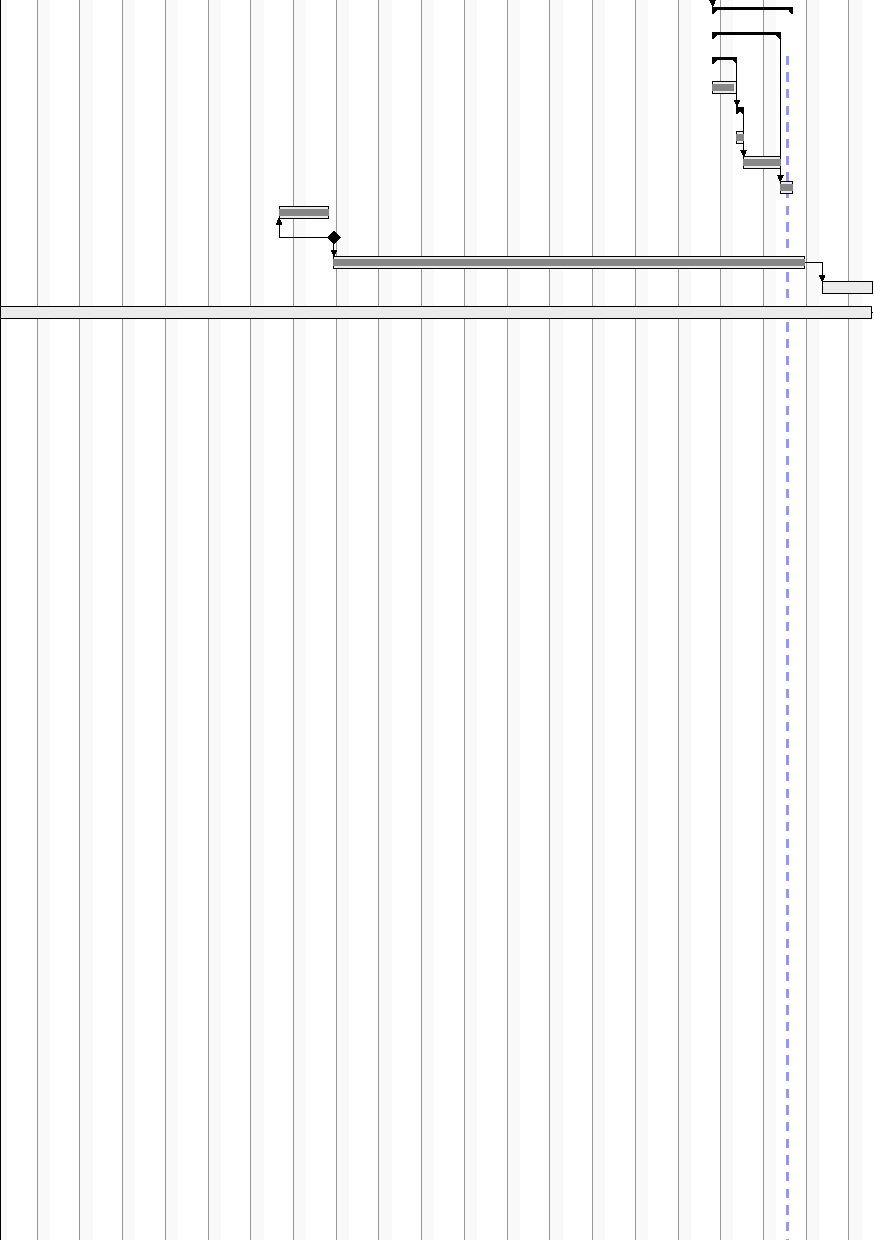
\includegraphics[width=1\textwidth]{gantt_nuevo_v_pag4}
	\end{fullpage}
	\caption[Final del Gantt, dreta]{\textbf{Final del Gantt, dreta} : Septembre, Octubre, Novembre, Desembre, Gener}
	\label{gantt_nuevo_v_pag4}
\end{figure}
  

\clearpage

%: ----------------------- HELP: references
% References can be links to figures, tables, sections, or references.
% For figures, tables, and text you define the target of the link with \label{XYZ}. Then you call cross-link with the command \ref{XYZ}, as above
% Citations are bound in a very similar way with \cite{XYZ}. You store your references in a BibTex file with a programme like BibDesk.


% ----------------------------------------------------------------------



